\documentclass[a4paper]{article}

\usepackage[swedish]{babel}
\usepackage[T1]{fontenc}
\usepackage[utf8]{inputenc}
\usepackage{graphicx}
\usepackage{array}
\usepackage[nottoc,notlot,notlof]{tocbibind}
\usepackage{appendix}
\usepackage{acro}
\usepackage[dvips]{graphicx}
\usepackage{float}

\begin{document}

\pagenumbering{gobble}
\title{\textbf{Utveckling och konstruktion av larmsystem med MD407-enheter} \newline \newline \large Larmsystem med centralenhet, dörrlarmsenhet, rörelselarmsenhet samt en störenhet för teständamål}
\author{Daniel Ferriera, Christoffer Kaltenbrunner, \\Lam Nguyen, Erik Söderpalm, Jakob Wik}
%\date{datum goes here}
\maketitle

\begin{center}
Datateknik, DAT290
\end{center}

\begin{table}
\centering
\begin{tabular}{|c|c|c|}   \hline
         & Namn & Datum \\ \hline
Granskad &      &       \\ \hline
Godkänd  &      &       \\ \hline
\end{tabular}
\end{table}

\newpage

\pagenumbering{roman}

\tableofcontents
\newpage

\pagenumbering{arabic}

\section{Introduktion}
Mellan 2017 och 2018 ökade säkerhetsbranschen med cirka 8 procent och omsatte 39 miljarder kronor i Sverige.
Detta beror inte på att brottsligheten ökar, utan på att fler svenskar upplever att brottsligheten ökar,
menar Jerzy Sarnecki, professor i kriminologi\cite{sverigesRadio}. För att fler svenskar ska uppleva en förhöjd känsla av säkerhet behöver ett tryggt och användarvänligt larmsystem etableras på marknaden.

\subsection{Syfte}

Projektet syftar till att utveckla och konstruera ett larmsystem
som bidrar till att fler svenskar upplever en förhöjd känsla av säkerhet i sina hem.

\subsection{Mål}

Målet med projektet är att utveckla ett larmsystem med hjälp av en mikrokontroller och ett antal periferienheter.
Larmsystemet, som består av ett grundsystem med ett antal tilläggsfunktioner, är effektivt och användarvänligt.

Grundsystemet utgörs av en centralenhet, en dörrlarmsenhet (periferienhet 1), en rörelselarmsenhet (periferienhet 2) samt en störenhet. Inställningarna för de två periferienheterna kan konfigureras via centralenheten.

Tilläggsfunktionerna delas in i två delar: (1) viktiga funktioner och (2) mindre viktiga funktioner. De viktiga funktionerna omfattar en funktion att slå om från produktionsläge till testläge för enklare test av periferienheterna samt en funktion som gör systemet självlärande.  De mindre viktiga funktionerna omfattar    kryptering av meddelanden som skickas i systemet samt framtagandet av en uppseendeväckande larmsignal.

\subsection{Arbetsmetod}

Som grund för arbetet med projektet ligger en tidsplan och ett antal milstolpar som tagits fram vid projektets uppstart. För att kontinuerligt stämma av hur väl projektets delmål uppnås sker regelbundna möten där samtliga gruppmedlemmar förväntas deltaga. Vid behov kan resurser omfördelas för att nå projektets delmål.

Tidsplanen är ingen detaljplanering, utan en överblicksplanering, som används för att fördela resurser inför den kommande veckan. Detta är fördelaktigt då det kan vara svårt att detaljplanera hur arbetet ska utföras innan det är kännt vilka förutsättningar som råder när arbetet ska utföras.

\subsubsection{Versionshantering}
För projektet har versionshanteringssystemet \textit{Git} använts. All kod finns tillgänglig på ett fjärrarkiv på \textit{GitHub}.

\subsubsection{Dokumentation}

Projektet är dokumenterat genom möteskallelser och -protokoll samt genom att använda \textit{Issue}-funktionen på GitHub. För buggrapportering, frågor och återkoppling om dokumentation eller kod, samt granskning av testfall, öppnas ett ärende (\textit{eng.} issue) på GitHub. Diskussionen kring ett ärende sker i ärendets kommentarsfält. Samtliga öppna ärenden tas upp på veckomötena där de diskuteras och nästa steg bestäms. Det som diskuteras på ett veckomöte dokumenteras sedan i ärendets kommentarsfält. Genom att samla alla projektets problem (buggar) och frågor på samma ställe kan samtliga gruppmedlemmar och kunden få en övergripande bild av vad som inte fungerar, vart projektet är på väg och vad som måste göra. 

\subsubsection{Mjukvaruutveckling och testning}

Under projektet implementeras de krav som kunden ställt på grundsystemet (se tabell \ref{tabell:krav} på sida \pageref{tabell:krav}). För att kontrollera att kraven uppnås - och därmed kvalitetssäkra produkten - skrivs och utförs ett testfall för varje krav. Om det körda testet blir godkänt är kravet uppnått.

Under mjukvaruutvecklingen integreras utveckling med testning för att kunna leverera en högkvalitativ produkt. För att så tidigt som möjligt i utvecklingsfasen hitta och lösa buggar testas en funktion (ej att förväxla med krav) så fort den har utvecklats. Dessa tester utförs i första hand i hårdvaran, men vid behov används en simulator. Fördelen med att testa direkt i hårdvaran är att det som fungerar i en simulator inte nödvändigtvis behöver fungera i hårdvaran, vilket skapar ett extra teststeg.

\subsubsection*{Funktionella tester och användartester}

I projektet utförs funktionella tester som testar funktionaliteten av olika delar av systemet, prestandatester för att fastställa systemets prestanda och kapacitet, samt användartester för att upptäcka förbättringar av systemet utifrån ett användarperspektiv. Varje testfall består av följande data:

\begin{description}
  \item [ID] Ett unikt ID på formen TXnnnvm, där X är F, P eller A för funktionellt test, prestandatest respektive användartest, nnn är ett nummer mellan 0 och 999 tilldelat i den ordning testfallen skapats, och m är versionsnummret. Exempelvis är TF012v3 den tredje versionen av det tolfte funktionella testfallet.
  \item [Namn] Ett namn som tydligt beskriver vad testfallet ska testa.
  \item [Beskrivining] En beskrivning av testfallet. Beskrivningen ska beskriva syftet med testfallet, vilken komponent som testas, vilket eller vilka krav som testas samt eventuella tekniska förutsättningar för att genomföra testet.
  \item [Teststeg] De steg som måste utföras för att utföra testfallet.
  \item [Förväntat resultat] Beskrivning av det förväntade resultatet för testfallet.
\end{description}

\noindent
Eftersom produkten kvalitetssäkras av tester är det självklart viktigt att kvalitén på testfallen och utförandet av dem är mycket hög. För att säkerställa att alla testfall som skrivs håller en hög kvalité sker skapandet och utförandet av testfallen enligt följande rutin:

\begin{enumerate}
\item När ett testfall skapas tilldelas det automatiskt status \textit{Utkast}. Testfallet kan sedan skickas vidare till \textit{granskning}.
\item Granskningen ska ske av åtminstone en (1) person och personen får inte ha varit inblandad i skrivandet av testfallet. Testfallet kan antingen bli \textit{godkänt} eller \textit{avfärdat}.
\item Om testfallet blir godkänt ändras dess status till \textit{Klar för test} och det får köras. Om testfallet däremot blir avfärdat måste det revideras och sedan åter skickas till granskning.
\item Ett föråldrat eller inaktuellt testfall med status \textit{Klar för test} kan skickas tillbaka till granskning.
\end{enumerate}

\noindent
Denna rutin visualiseras i figur 1.

De två reglerna för att skapa och köra testfall är följande: (1) endast testfall med status \textit{Utkast} får redigeras och (2) endast testfall som har blivit granskade och godkända får köras.

\begin{figure}[h]
  \centering
  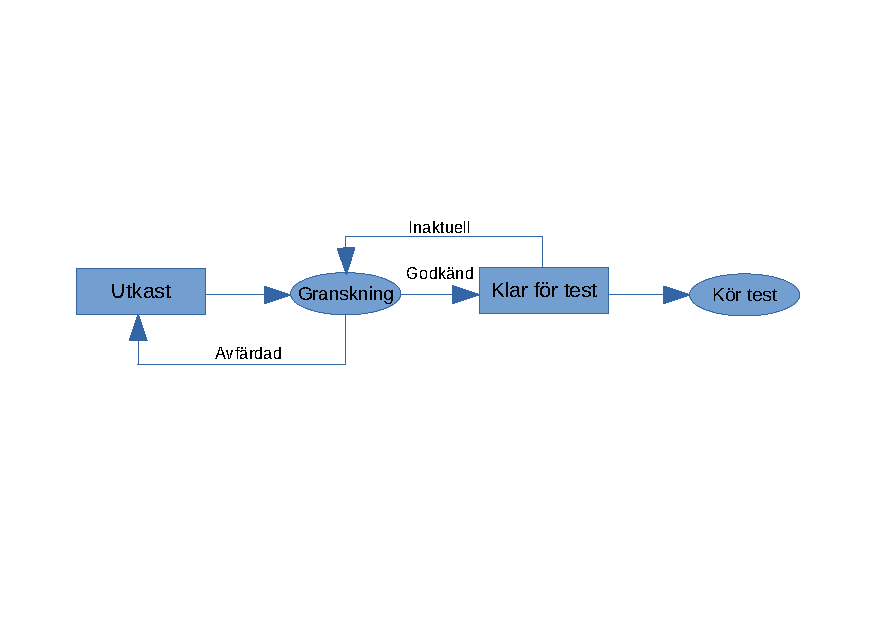
\includegraphics[trim={0 4cm 0 3cm}, clip, scale=0.8]{figurer/testrutin.pdf}
  \caption{Rutin kring att skriva och genomföra testfall.}
\end{figure}

\noindent
Samtliga körda testfall är samanställda i appendix A och resultatet av samtliga körda tester är sammanställda i appendix B.


\newpage

\section{Teknisk beskrivning}
\input{teknisk_beskrivning.tex}
\newpage

\section{Resultat}
I detta kapitel sammanställs projektets resultat.

\subsection{Larmsystemet}
Ett larmsystem utifrån kraven i tabell \ref{tabell:krav} har konstruerats. Dessutom har två ytterligare funktioner implementerats: en funktion att slå om från produktionsläge till testläge och en funktion att kryptera meddelanden som skickas mellan enheterna.

\subsection{Testresultat}

Samtliga körda tester på den sista versionen av mjukvaran har blivit godkända.  Detta innebär att samtliga krav för grundsystemet är verifierade och produkten är kvalitetssäkrad. Samtliga tester är sammanställda i appendix A och resultatet av samtliga körda tester är sammanställda i appendix B.

Två prestandatester för systemet har utförts. Det ena har testat rörelsemätarens räckvidd med resultatet att räckvidden är ungefär tre meter. Det andra har testat hur väl systemet klarar belastning från störenheten med resultat att cirka 50 meddelanden kan skrivas ut i PC:ns terminalfönster innan det hänger sig.


\newpage

\section{Diskussion}
\label{sec:Diskussion}
Detta kapitel diskuterar de olika systemens designval, huruvida projektets tidsplan varit till fördel eller inte, samt möjliga förbättringar av systemet.

\subsection{Projektets tidsplan}

Enligt projektets mål och tidsplan var förhoppningen att
systemet skulle ha ett antal tilläggsfunktioner, varav två har utvecklats.
Anledningen till att inte fler utvecklats beror i stort på två faktorer, vilka är en felaktig fördelning 
av arbetsuppgifter och en feluppskattning av den tid som krävdes för att utveckla grundsystemet. 
En felaktig fördelning av arbetsuppgifter innebär att strategin att utveckla delar av systemet i kodlag, om två personer per lag, inte fungerade, ty en arbetstimme är lika med två mantimmar.

Det är svårt att avgöra om larmsystemet hade haft exempelvis ett bättre användargränssnitt, eller fler konfigurationsmöjligheter för användaren, ifall en bättre fördelning av arbetsuppgifterna hade förekommit. 
Alternativt om projektets mål var för högt satta i förhållande till 
den tidsram som de skulle uppnås i. Trots detta ses den övergripliga tidsplanen, vilken låg som grund för projektet, fortfarande som något positivt. Den gav utrymme för motgångar i utvecklingen och satte mindre press på utvecklarna.

\subsection{CAN: Säkerhetsrisk och tänkbara åtgärder}

CAN är ett enkelt kommunikationssystem som uppfyller kraven för snabbhet, men CAN:s brist i säkerhet lämnar mycket övrigt att önska. Exempelvis om en inkräktare har fysisk tillgång till databussen så har den direkt åtkomst till all kommunikation i nätverket. Inkräktaren har då möjlighet att läsa av och förfalska meddelanden eller blockera en enhet med en \textit{Denial-of-service}-attack (DoS).

Störenheten är uppbyggd kring just denna svaghet. Den här typen av attack är enkel att utföra men svår att avstyra. 
Med hjälp av meddelandefilter kan en enhet filtrera oönskade meddelanden, vilket inte räcker till för att skydda enheten mot en återuppspelnings-attack (\textit{eng.} replay-attack). Återuppspelnings-attackens svaghet är att den inte påbörjas förrän den hittar något meddelande att förfalska. Ett skyddssystem för nätverk som använder CAN kan utvecklas kring den här svagheten. Om en enhet i ett CAN-kommunikationsnätverk blockerar meddelandets ID direkt efter mottagning kommer det förfalskade meddelandet från inkräktaren inte ha någon effekt, eftersom det kommer att filtreras bort. Men då måste ett nytt ID tilldelas till den enheten så att andra riktiga enheter i nätverket kan skicka till den utan att framtida meddelanden också blir filtrerade. Det nya ID:t ska vara förbestämt eller medskickat i meddelandet så att enheterna känner till varandras ID:n utan direkt kommunikation.

En annan svaghet med CAN är att alla meddelanden tas emot av samtliga noder som befinner sig i nätverket. Därför är krypteringen av meddelandet ett väsentligt krav. Vårt system använder sig av en egenbyggd krypteringsalgoritm som roterar alla bitar i meddelandets datafält ett antal steg åt höger. Antal steg bestäms beroende på meddelandets ID-fält. Detta innebär att antalet steg varierar, vilket försvårar dekrypteringsförsök utan tillkännande av algoritmen och meddelandets ID-fält. 

Dessa skydd minskar risken för ett CAN-kommunikationssystem, men det behåller ändå viktiga egenskaper.

\subsection{Konstruktion av störenheten}

CAN-bussen kan konfigureras till att hantera en datamängd upp till och med 1 Mbps. Störenheten kan blockera kommunikationen mellan enheterna genom att skicka den mängden data med högsta meddelandeprioritet på CAN-bussen. Störenheten blockerar då all övrig kommunikation på nätverket.

Störenheten använder sig också av återspeglings-attacker för att störa andra enheter på nätverket. Den är konstruerad att hela tiden jämföra infångade meddelandens prioriteringar med varandra och förfalska dem med högst prioritet. Därmed har störenheten möjlighet att blockera kommunikationen till och från en viktig enhet i nätverket. Nackdelen med denna typ av attack är att den inte börjar förrän något meddelande skickas på CAN-bussen. Vidare om det fångade meddelandet har ett blockerat ID misslyckas attacken.

\subsection{Fördelar med avbrott}

Alla tidskritiska händelser i systemet genererar ett avbrott. Det som är fördelaktigt med detta är att processorn hanterar händelsen i den stund den sker, istället för om det legat i huvudprogrammet och utförs i en viss ordning. Allt som inte är tidskritiskt hanteras av respektive enhets huvudprogram.

Så lite som möjligt ska ske i en avbrottsrutin: nödvändiga initieringar, sätta en flagga och kvittera avbrottet. Resten hanteras av huvudprogrammet. På så sätt undviks att hela systemet kan komma att sluta fungera på grund av en \textit{busy wait}.

\subsection{Möjliga förbättringar av systemet}

Nedan redogörs för ett antal möjliga förbättringar av systemet.

\subsubsection*{Ping}

Ett problem med ping-funktionen som den nu är implementerad är att om samtliga enheter kopplas från nätverket så slutar centralenheten att larma. Detta beror på att centralenheten inte kan skicka ut några meddelanden på nätverket eftersom det inte finns några mottagarnoder. Den enklaste lösningen på problemet vore att låta alla enheter på nätverket med ett bestämt tidsintervall pinga centralenheten istället för tvärtom. Om samtliga enheter kopplas från nätverket kommer nu centralenheten att larma.

\subsubsection*{Bekräftelse av meddelanden}

För denna version av systemet bekräftas inte meddelanden som skickas på nätverket. Detta innebär att om ett meddelande, av någon anledning, inte kommer fram till mottagaren, så är meddelandet förlorat. För att lösa problemet bör en bekräftelse på varje mottaget meddelande skickas från mottagaren till sändaren. Om sändaren inte mottager en bekräftelse inom en viss tid så skickas meddelandet igen.

Detta skulle även lösa ett problem då larm för flera enheter uppstår samtidigt. CAN har nämligen bara stöd för upp till och med tre stycken inkorgar. Om fler än tre larm kommer samtidigt så går de sista förlorade. I ett system som bekräftar meddelanden kommer de tre första meddelanden att bekräftas. Resterande meddelanden kommer att skickas av sändaren igen, tills samtliga meddelanden bekräftats.

\subsubsection*{Okänd aktivitet på nätverket}

Antag att centralenheten stödjer upp till och med $n$ enheter på nätvärket och att den är konfigurerad för $m < n$ enheter. Om en enhet med ID $i$ så att $m < i <= n$ kopplas upp på nätverket och ett larm startas från den enheten, så kommer centralenheten att larma för enhet $i$. Det är användarens ansvar att konfigurera systemet för endast de enheterna som används. Dock kan detta lösas genom att centralenheten, innan den larmar, kontrollerar att den faktiskt är konfigurerad för att stödja enheten som larmar. Om inte, så larmar den för att den upptäckt okänd aktivitet på nätverket.

\subsubsection*{Prioritering för meddelandetyper}

Ping-meddelanden har id 0x4, vilket är högre än både kommando-meddelanden och konfigurationsmeddelanden, 0x2 respektive 0x3. I nästa version av systemet bör ping-meddelanden ha högre prioritet än de andra ovan nämnda meddelandetyperna.

\subsubsection*{Rörelselarmsenheten}

Rörelsedetektorn är konstruerad så att den fyra gånger i sekunden mäter tiden, $t_{i}$, det tar för ultraljudet att komma tillbaka till enheten. Därefter beräknas sträckan, $s_{i}$, som ultraljudet rört sig. Denna sträcka jämförs med sträckan vid mätningen innan, $s_{i-1}$. Om skillnaden, $d = | s_{i} - s_{i-1} |$, överskrider ett visst värde går larmet. Ultraljudsmätaren kalibreras vid uppstart av systemet vilket innebär att $t_{0}$ beräknas. Därefter går programmet in i huvudloopen där $t_{1}$ beräknas och jämförs med $t_{0}$.

Ett motargument till detta sätt att konstruera rörelselarmsenheten är att eftersom varje mätning jämförs med mätningen som gjordes gången innan så kan någon långsamt smyga fram till sensorn och ställa en låda framför utan att larmet går. Noggranna tester av rörelselarmet visar att med rätt känslighet inställd går inte detta.

Detta sätt att konstruera rörelselarmet tillåter att något rör sig en viss sträcka under en viss tid. Genom att ställa in rätt känslighet är detta inte en säkerhetsrisk. Ett annat sätt att konstruera enheten på vore att alltid jämföra den senast mätta sträckan med initieringsvärdet så att $d = | s_{i} - s_{0} |$.

För att undvika felmätningar bör ultraljudsmätaren mäta flera gånger vid varje mätning, exempelvis fem mätningar och använda medianen av dessa.


\subsubsection*{Förslag efter användartest}

Ett användartest har med godkänt resultat utförst på hela systemet. Testarens kommentar anger att samtliga enheter bör skriva ut enhets-information, till exempel enhets-ID och typ av enhet, vid uppstart.

\newpage

\section{Slutsats}
Sammanfattninsvis dras slutsatsen att larmsystemet har stor utvecklingspotential i form av ytterligare tilläggsfunktioner samt förbättrad säkerhet för CAN-kommunikationen, som diskuterats tidigare. 

Icke desto mindre är samtliga krav som ställdes på grundsystemet uppfyllda. Därmed uppfyller det framställda larmsystemet projektets syfte och mål, vilka var att utveckla och konstruera ett larmsystem som bidrar till en förhöjd känsla av säkerhet hos befolkningen.


\newpage

\appendix
\section{Tester}
\label{sec:app_a}
\begin{table}[h!]
\begin{tabular}{| p{0.18\linewidth} | p{0.72\linewidth} |}
\hline
\textbf{ID} & TF001v1 \\ \hline
\textbf{Namn} & Test av dörrlarm\\ \hline
\textbf{Beskrivning} & Syfte: Verifiera att dörrlarmet fungerar enligt spefikation i projektrapporten. \newline
Komponent: P1 (steg 1-3) och C (steg 4-5) \newline
Krav: K01 (steg 1-3) och K02 (steg 4-5) \\ \hline
\textbf{Teststeg} & 1. Låt dörren stå öppen. \newline
2. Vänta tills enheten larmar lokalt. \newline
3. Vänta tills enheten larmar centralenheten. \newline
4. Mata in fel kod på centralenhetens knappsats. \newline
5. Mata in rätt kod på centralenhetens knappsats. \newline
6. Upprepa setg 1-5 flera gånger. \\ \hline
\textbf{Förväntat resultat} & Efter en viss tid ska enheten larma lokalt, dvs. en röd lysdiod ska tändas. 
Efter ytterligare en viss tid ska enheten larma centralenheten.
När fel kod matas in ska larmet fortsätta.
När rätt kod matas in ska larmet sluta.
\\ \hline
\end{tabular}
\end{table}

\begin{table}[h!]
\begin{tabular}{| p{0.18\linewidth} | p{0.72\linewidth} |}
\hline
\textbf{ID} & TF002v1 \\ \hline
\textbf{Namn} & Inaktivering och aktiviering av dörrlarm \\ \hline
\textbf{Beskrivning} & Syfte: Verifiera att inaktivering och aktivering av dörrlarm fungerar. \newline
Komponent: P1 \newline
Krav: K06 \\ \hline
\textbf{Teststeg} & 1. Inaktivera larmet på en dörr. \newline
2. Ställ upp dörren. \newline
3. Vänta.\newline
4. Stäng dörren.\newline
5. Aktivera dörrlarmet.\newline
6. Ställ upp dörren.\newline
7. Vänta tills larmet går.\newline
8. Stäng av larmet.\newline
9. Upprepa steg 1-8 flera gånger.\\ \hline
\textbf{Förväntat resultat} & När larmet är inaktiverat ska en grön lysdiod lysa på centralenheten och larmet
INTE gå när dörren står öppen.
När larmet är aktiverat ska larmet gå när dörren står öppen.
\\ \hline
\end{tabular}
\end{table}

\newpage

\begin{table}[h!]
\begin{tabular}{| p{0.18\linewidth} | p{0.72\linewidth} |}
\hline
\textbf{ID} & TF003v1 \\ \hline
\textbf{Namn} & Konfigurering av tid en dörr tillåts vara öppen \\ \hline
\textbf{Beskrivning} &
Syfte: Verifiera att tiden en dörr tillåts vara öppen kan ändras via 
centralenheten.\newline
Komponent: P1 och C\newline
Krav: K06
\\ \hline
\textbf{Teststeg} &
1. Konfigurera tiden en dörr tillåts vara öppen via centralenheten. \newline
2. Öppna dörren. \newline
3. Vänta tills larmet går. \newline
4. Upprepa steg 1-3 flera gånger med olika tider.
\\ \hline
\textbf{Förväntat resultat} & Efter att tiden som konfigurerats via centralenheten passerat ska larmet gå.
\\ \hline
\end{tabular}
\end{table}

\begin{table}[h!]
\begin{tabular}{| p{0.18\linewidth} | p{0.72\linewidth} |}
\hline
\textbf{ID} & TF004v1 \\ \hline
\textbf{Namn} & Test av avståndsmätare, rörelselarm \\ \hline
\textbf{Beskrivning} &
Syfte: Verifiera att avståndsmätaren i rörelselarmet fungerar enligt
specifikationen i projektrapporten. \newline
Komponent: P2\newline
Krav: K07
\\ \hline
\textbf{Teststeg} &
1. Kalibrera avståndsmätaren.\newline
2. Ställ in känslighet.\newline
3. Gå inom känslighetsområdet för avståndsmätaren.\newline
3. Upprepa steg 2-3 med olika känslighet.
\\ \hline
\textbf{Förväntat resultat} & Larmet ska gå när någon rör sig inom avståndsmätarens känslighetsområde.
\\ \hline
\end{tabular}
\end{table}

\begin{table}[h!]
\begin{tabular}{| p{0.18\linewidth} | p{0.72\linewidth} |}
\hline
\textbf{ID} & TF005v1 \\ \hline
\textbf{Namn} & Test av vibrationssensor, rörelselarm \\ \hline
\textbf{Beskrivning} &
Syfte: Verifiera att vibrationssensorn i rörelselarmet fungerar enligt
specifikationen i projektrapporten.\newline
Komponent: P2\newline
Krav: K09
\\ \hline
\textbf{Teststeg} &
1. Ställ in känsligheten för vibrationssensorn.\newline
2. Simulera att en glasruta krossas.\newline
3. Upprepa steg 1-2 med olika känslighet för vibrationssensorn.
\\ \hline
\textbf{Förväntat resultat} & När simuleringen av att en glasruta krossas sker, ska larmet gå.
\\ \hline
\end{tabular}
\end{table}

\newpage

\begin{table}[h!]
\begin{tabular}{| p{0.18\linewidth} | p{0.72\linewidth} |}
\hline
\textbf{ID} & TF006v1 \\ \hline
\textbf{Namn} & Test av nätverket\\ \hline
\textbf{Beskrivning} &
Syfte: Testa nätverkets funktion vid olika belastningsgrader.\newline
Komponent: Nätverk\newline
Krav: Saknas
\\ \hline
\textbf{Teststeg} &1. Anslut en störenhet till nätverket.\newline
2. Justera datavolymen störenheten ska skicka.\newline
3. Starta störenheten.\newline
4. Upprepa steg 2-3 med olika datavolym.
\\ \hline
\textbf{Förväntat resultat} & Nätverket ska klara en hög databelastning.
\\ \hline
\end{tabular}
\end{table}

\begin{table}[h!]
\begin{tabular}{| p{0.18\linewidth} | p{0.72\linewidth} |}
\hline
\textbf{ID} & TF007v1 \\ \hline
\textbf{Namn} & Test av centralenheten, uppstart\\ \hline
\textbf{Beskrivning} &
Syfte: Verifiera att centralenheten känner till anslutna enheter och deras konfigurering vid uppstart. \newline
Komponent: C\newline
Krav: K12
\\ \hline
\textbf{Teststeg} &
1. Verifiera att centralenheten känner till anslutna enheter och deras 
konfiguration vid uppstart.
\\ \hline
\textbf{Förväntat resultat} & Se teststeg 1.
\\ \hline
\end{tabular}
\end{table}

\begin{table}[h!]
\begin{tabular}{| p{0.18\linewidth} | p{0.72\linewidth} |}
\hline
\textbf{ID} & TF009v1 \\ \hline
\textbf{Namn} & Test av centralenheten, periferienhet kopplas från nätverket\\ \hline
\textbf{Beskrivning} &
Syfte: Verifiera att centralenheten larmar om en periferienhet kopplas från nätverket.\newline
Komponent: C\newline
Krav: K13
\\ \hline
\textbf{Teststeg} &
1. Anslut en periferienhet till nätverket.\newline
2. Koppla bort periferienheten från nätverket genom att dra ut 
strömförsörjningsadaptern.
\\ \hline
\textbf{Förväntat resultat} & Centralenheten ska larma.
\\ \hline
\end{tabular}
\end{table}

\newpage

\begin{table}[h!]
\begin{tabular}{| p{0.18\linewidth} | p{0.72\linewidth} |}
\hline
\textbf{ID} & TF011v1 \\ \hline
\textbf{Namn} & Test av centralenheten larmfunktion (1/2)
\\ \hline
\textbf{Beskrivning} &
Syfte: Verifiera att när ett larm uppstår kommunicerar centralenheten det till en ansluten PC via USART.\newline
Komponent: C och P1\newline
Krav: K11
\\ \hline
\textbf{Teststeg} &
1. Starta ett larm från P1.\newline
2. Upprepa steg 1 med samtliga olika sätt att starta larm på.
\\ \hline
\textbf{Förväntat resultat} & När larmet går kommunicerar centralenheten detta till en ansluten PC.
\\ \hline
\end{tabular}
\end{table}

\begin{table}[h!]
\begin{tabular}{| p{0.18\linewidth} | p{0.72\linewidth} |}
\hline
\textbf{ID} & TF012v1 \\ \hline
\textbf{Namn} & Test av centralenheten larmfunktion (2/2)
\\ \hline
\textbf{Beskrivning} &
Syfte: Verifiera att när ett larm uppstår kommunicerar centralenheten det till en ansluten PC via USART. \newline
Komponent: C och P2\newline
Krav: K11
\\ \hline
\textbf{Teststeg} &
1. Starta ett larm från P2.\newline
2. Upprepa steg 1 med samtliga olika sätt att starta larm på.
\\ \hline
\textbf{Förväntat resultat} & När larmet går kommunicerar centralenheten detta till en ansluten PC.
\\ \hline
\end{tabular}
\end{table}

\begin{table}[h!]
\begin{tabular}{| p{0.18\linewidth} | p{0.72\linewidth} |}
\hline
\textbf{ID} & TF013v1 \\ \hline
\textbf{Namn} & Test av centralenheten larmfunktion (2/2)
\\ \hline
\textbf{Beskrivning} &
Syfte: Verifiera att flera dörrar kan larmas med samma enhet.\newline
Komponent: P1\newline
Krav: K03
\\ \hline
\textbf{Teststeg} &
1. Larma flera dörrar från P1.\newline
2. Upprepa steg 1 med olika antal dörrar.
\\ \hline
\textbf{Förväntat resultat} & Flera dörrar ska kunna larmas med samma enhet.
\\ \hline
\end{tabular}
\end{table}

\begin{table}[h!]
\begin{tabular}{| p{0.18\linewidth} | p{0.72\linewidth} |}
\hline
\textbf{ID} & TF014v1 \\ \hline
\textbf{Namn} & 
Test av flera dörrenheter på nätverket.
\\ \hline
\textbf{Beskrivning} &
Syfte: Verifiera att flera dörrenheter kan kopplas upp på nätverket.\newline
Komponent: N, P1\newline
Krav: K04
\\ \hline
\textbf{Teststeg} &
1. Koppla upp flera dörrlarmsenheter på nätverket.\newline
2. Verifiera att samtliga dörrlarmsenheter fungerar.
\\ \hline
\textbf{Förväntat resultat} & Samtliga dörrlarmsenheter ska fungera.
\\ \hline
\end{tabular}
\end{table}

\newpage

\begin{table}[h!]
\begin{tabular}{| p{0.18\linewidth} | p{0.72\linewidth} |}
\hline
\textbf{ID} & TF015v1 \\ \hline
\textbf{Namn} & 
Test av konfiguration av antalet dörrar på P1.
\\ \hline
\textbf{Beskrivning} &
Syfte: Verifiera att antalet dörrar för en dörrlarmsenhet kan konfigureras.\newline
Komponent: P1\newline
Krav: K05
\\ \hline
\textbf{Teststeg} &
1. Konfigurera antalet dörrar för en dörrlarmsenhet vid uppstart.
\\ \hline
\textbf{Förväntat resultat} & Antalet dörrar ska kunna konfigureras.
\\ \hline
\end{tabular}
\end{table}

\begin{table}[h!]
\begin{tabular}{| p{0.18\linewidth} | p{0.72\linewidth} |}
\hline
\textbf{ID} & TF016v1 \\ \hline
\textbf{Namn} & 
Test av kalibrering och känslighetsjustering av rörelsemätaren.
\\ \hline
\textbf{Beskrivning} &
Syfte: Verifiera känsligheten för rörelsemätaren kan ställas in samt att den kan kalibreras.\newline
Komponent: P2 och C\newline
Krav: K08
\\ \hline
\textbf{Teststeg} &
1. Kalibrera rörelsemätaren från centralenheten.\newline
2. Ställ in känsligheten för rörelsemätaren från centralenheten.\newline
3. Verifiera att rörelsemätaren är kalibrerad och har rätt känslighet.
\\ \hline
\textbf{Förväntat resultat} & Rörelsemätaren är kalibrerad och har rätt känslighet.
\\ \hline
\end{tabular}
\end{table}

\begin{table}[h!]
\begin{tabular}{| p{0.18\linewidth} | p{0.72\linewidth} |}
\hline
\textbf{ID} & TF017v1 \\ \hline
\textbf{Namn} & 
Test av störenheten
\\ \hline
\textbf{Beskrivning} &
Syfte: Verifiera att volymen data som störenheten skickar kan justeras.\newline
Komponent: S\newline
Krav: K10
\\ \hline
\textbf{Teststeg} &
1. Ändra volymen data som störenheten kan skicka.\newline
2. Verifiera att volymen data som störenheten skickar är ändrad.
\\ \hline
\textbf{Förväntat resultat} & Volymen data som störenheten skickar är ändrad enligt specifikation.
\\ \hline
\end{tabular}
\end{table}

\newpage
\begin{table}[h!]
\begin{tabular}{| p{0.18\linewidth} | p{0.72\linewidth} |}
\hline
\textbf{ID} & TF018v1 \\ \hline
\textbf{Namn} & 
Test av centralenhetens larmfunktion
\\ \hline
\textbf{Beskrivning} &
Syfte: Verifiera att centralenhetens larmar tills en fyrsiffrig kod knappas in på knappsatsen.\newline
Komponent: C\newline
Krav: K02
\\ \hline
\textbf{Teststeg} &
1. Starta larm.\newline
2. Vänta tills centralenheten larmar.\newline
3. Mata in fel fyrsiffrig kod.\newline
4. Mata in rätt fyrsiffrig kod.\newline
5. Upprepa steg 1-4 med olika larm.
\\ \hline
\textbf{Förväntat resultat} & Larmet ska fortsätta tills rätt kod matas in.
\\ \hline
\end{tabular}
\end{table}

\begin{table}[h!]
\begin{tabular}{| p{0.18\linewidth} | p{0.72\linewidth} |}
\hline
\textbf{ID} & TP001v1 \\ \hline
\textbf{Namn} & 
Rörelsesensorns räckvidd
\\ \hline
\textbf{Beskrivning} &
Syfte: Undersök räckvidden för rörelsesensorn.\newline
Komponent: P2\newline
Krav: Saknas
\\ \hline
\textbf{Teststeg} &
1. Undersök räckvidden för rörelsesensorn.
\\ \hline
\textbf{Förväntat resultat} & Se teststeg 1.
\\ \hline
\end{tabular}
\end{table}

\begin{table}[h!]
\begin{tabular}{| p{0.18\linewidth} | p{0.72\linewidth} |}
\hline
\textbf{ID} & TP001v1 \\ \hline
\textbf{Namn} & 
Störning på CAN-bussen
\\ \hline
\textbf{Beskrivning} &
Syfte: Undersöka hur mycket störning systemet klarar på CAN-bussen.\newline
Komponent: CAN-buss\newline
Krav: Saknas
\\ \hline
\textbf{Teststeg} &
1. Undersök hur mycket störning systemet klarar på CAN-bussen.
\\ \hline
\textbf{Förväntat resultat} & Se teststeg 1.
\\ \hline
\end{tabular}
\end{table}

\begin{table}[h!]
\begin{tabular}{| p{0.18\linewidth} | p{0.72\linewidth} |}
\hline
\textbf{ID} & TA001v1 \\ \hline
\textbf{Namn} & 
Test av systemet utifrån ett användarperspektiv
\\ \hline
\textbf{Beskrivning} &
Syfte: Verifiera att systemet har en god användarupplevelse.\newline
Komponent: P1, P2, C\newline
Krav: Saknas.
\\ \hline
\textbf{Teststeg} &
1. Starta upp systemet.\newline
2. Använd systemet.
\\ \hline
\textbf{Förväntat resultat} & Systemet ska ha en god användarupplevelse.
Kommentarer ska antecknas.
\\ \hline
\end{tabular}
\end{table}

\newpage

\newpage

\section{Testresultat}
\label{sec:app_b}
I detta appendix sammanställs det senaste testresultatet för samtliga körda tester för projektet. \textit{ID} är testfallets ID (se appendix A), \textit{Status} är anting godkänt (G) eller underkänt (U) och \textit{Kommentar} är en fritextkommentar som testaren kan ange.

\begin{table}[h!]
\begin{tabular}{| l | l | p{0.68\linewidth} |}
\hline
\textbf{ID} & \textbf{Status} & \textbf{Kommentar} \\ \hline
TF001v1 & G & \\ \hline
TF002v1 & G & En bargraph används istället för lysdioder för releasen. \\ \hline
TF003v1 & G & \\ \hline
TF004v1 & G & \\ \hline
TF005v1 & G & \\ \hline
TF006v1 & G & \\ \hline
TF007v1 & G & \\ \hline
TF009v1 & G & \\ \hline
TF010v1 & G & \\ \hline
TF011v1 & G & \\ \hline
TF012v1 & G & \\ \hline
TF013v1 & G & \\ \hline
TF014v1 & G & \\ \hline
TF015v1 & G & \\ \hline
TF016v1 & G & \\ \hline
TF017v1 & G & \\ \hline
TF018v1 & G & \\ \hline
TP001v1 & G & Ultraljudsmätaren har en räckvidd på ca 3 meter. \\ \hline
TP002v1 & G & Centralenheten klarar ca 50 meddelanden per sekund innan terminalfönstret hänger sig. Centralenheten kan inte larma av andra enheter medan den mottager meddelanden från störenheten. \\ \hline
TA001v1 & G & Alla enheter bör skriva ut enhets-info vid uppstart. \\ \hline
\end{tabular}
\end{table}

\newpage

\begin{thebibliography}{999}
\label{sec:referenser}
\bibitem{sverigesRadio}
L. Jungefeldt. ``Säkerhetsbranschen växer i Sverige`` sverigesradio.se. https://sverigesradio.se/sida/artikel.aspx?programid=83\&artikel=7284631 (hämtad 2019-09-07)
\bibitem{MD407}
F. Östman, ``MD407 - En ARM-baserad laborationsdator för utbildning``, Examensarbete, Inst. för data- och informationsteknik, Chalmers Tekniska Högskola, Göteborg, Sverige, 2016. [Online] Tillgänglig: https://hdl.handle.net/20.500.12380/232582
\end{thebibliography}



\end{document}


